\chapter{RESULTADOS E DISCUSSÃO}


Neste capítulo, são expostos todos os resultados alcançados até o momento ao longo do progresso do projeto, abrangendo ...

A montagem do protótipo pode ser vista na Figura \ref{fig:prototipo2}. 

\begin{figure}[H]
    \centering
    \captionsetup{justification=centering}
    \caption{Montagem física do protótipo vista em diagonal} 
    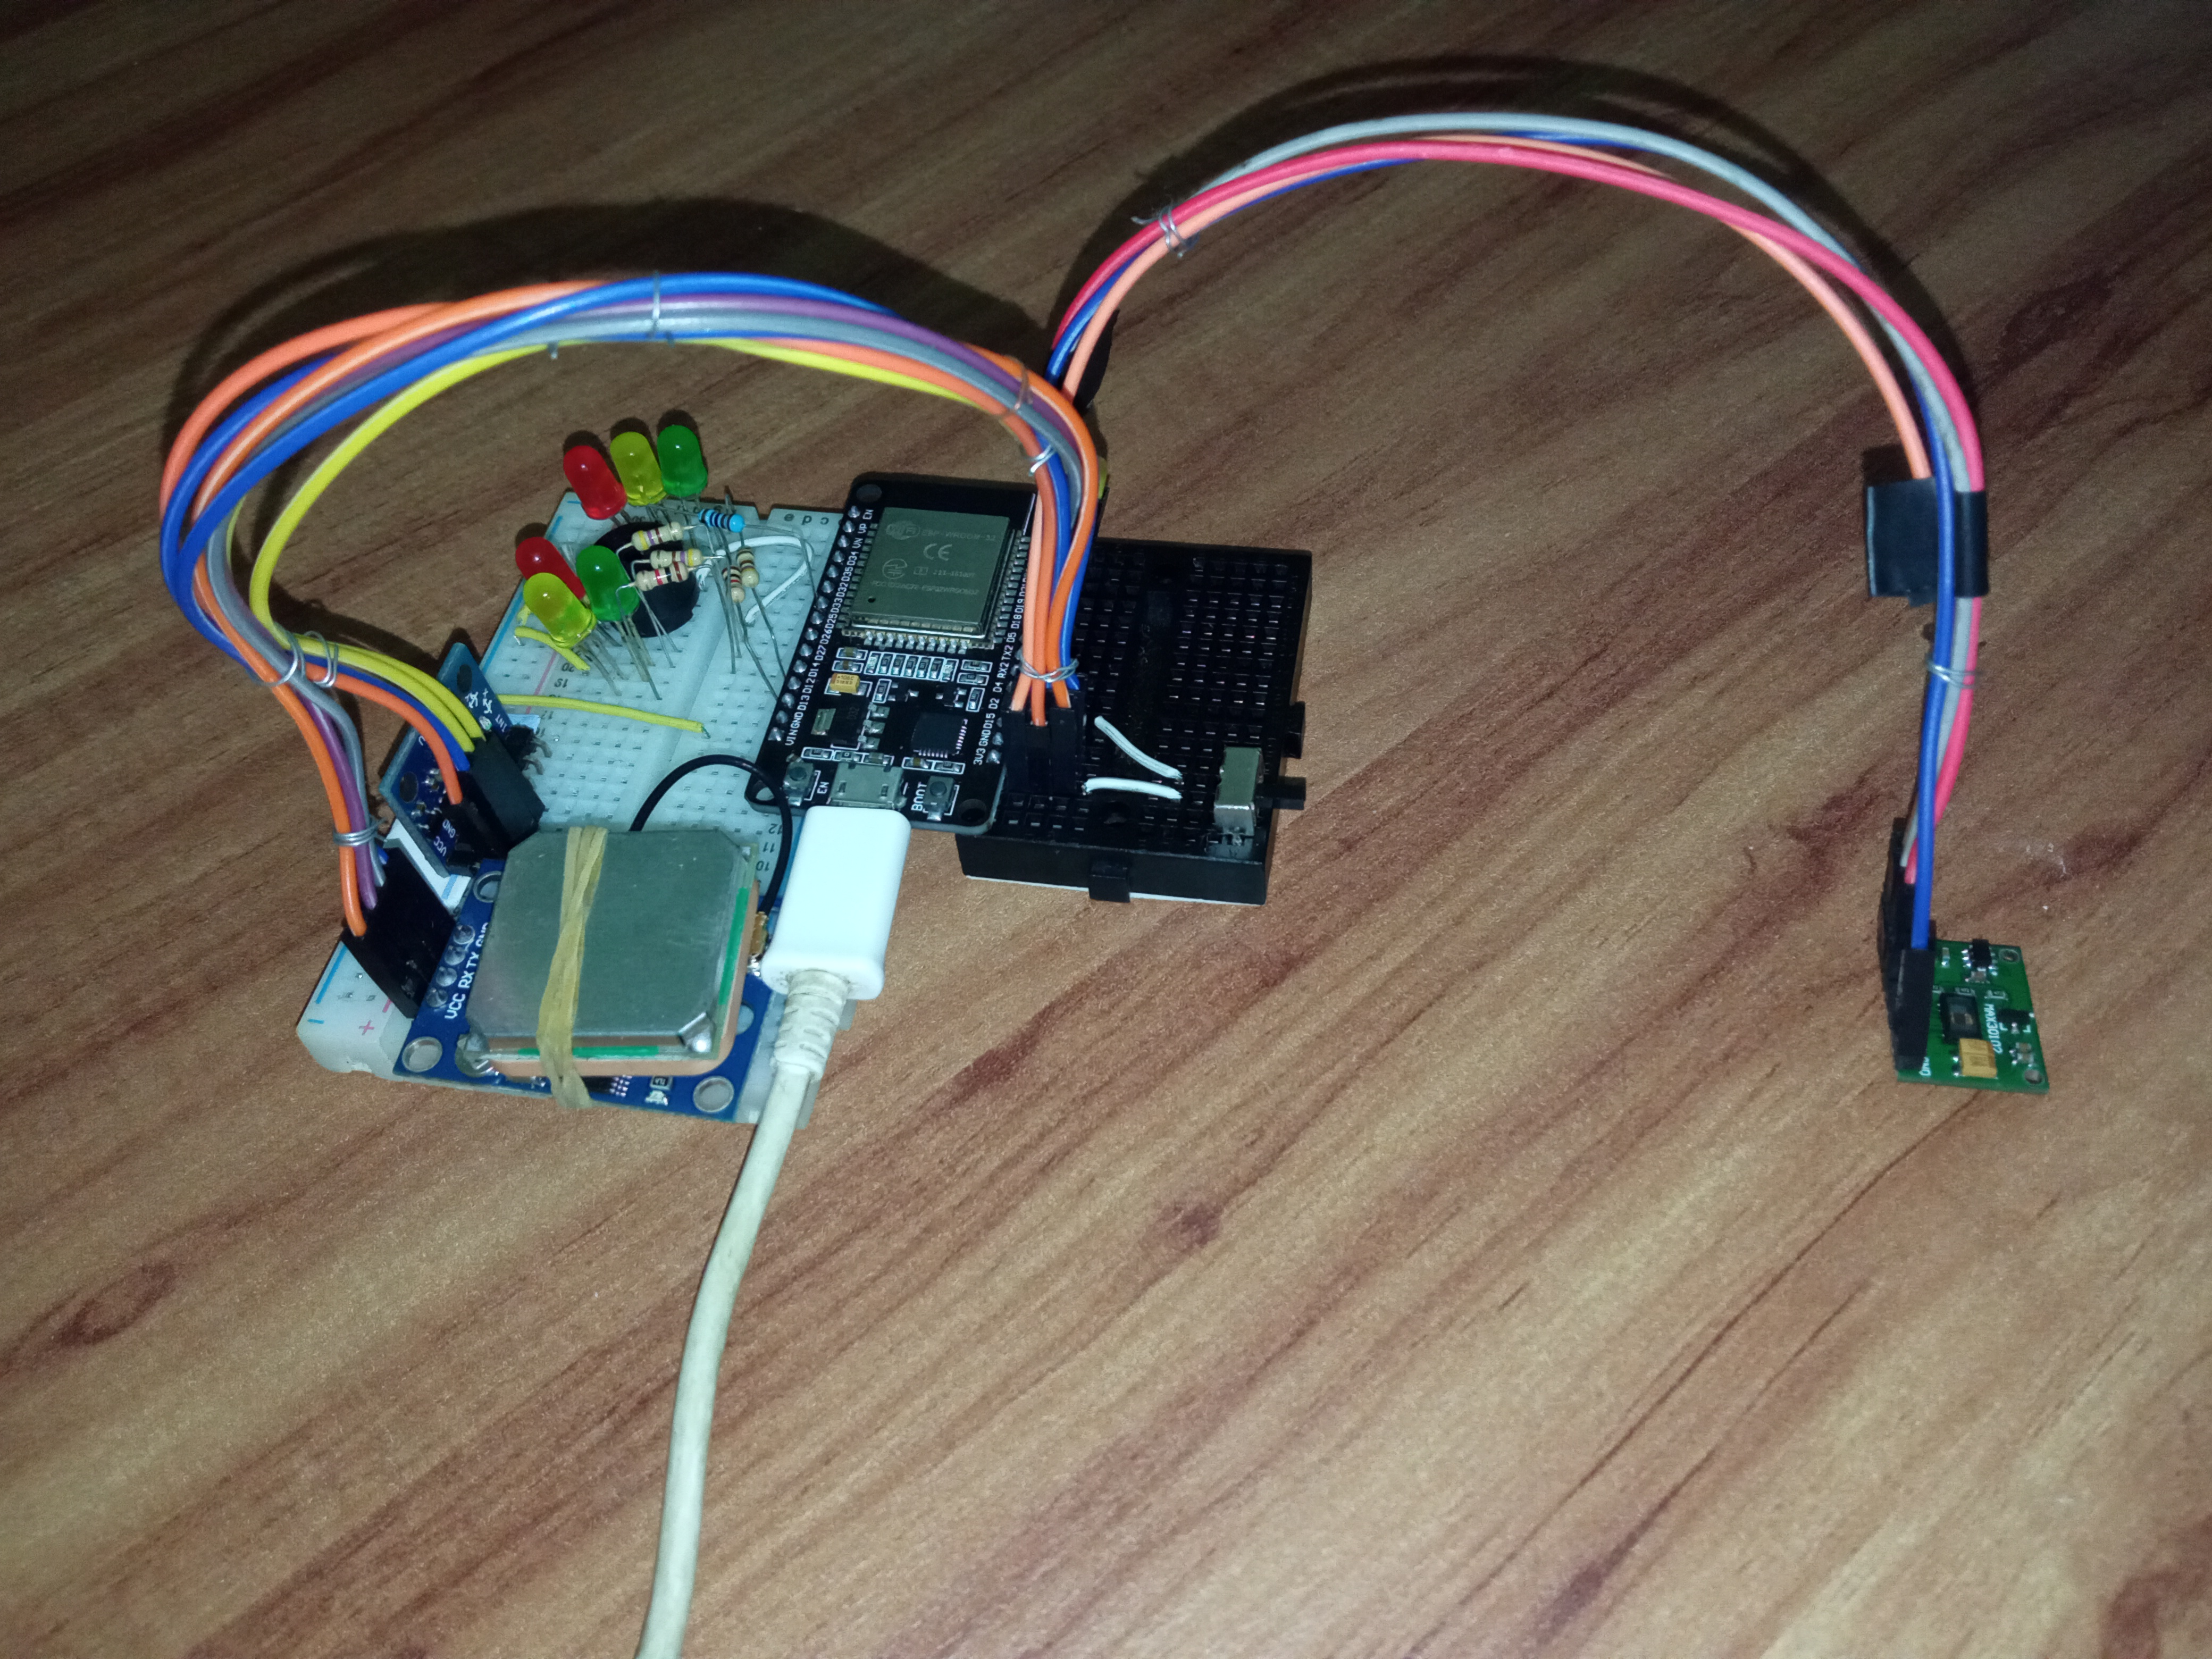
\includegraphics[width=0.7\textwidth]{figures/resultadosPrototipo/prototipo2.jpg}
    \legend{Fonte: Os autores, 2023}
    \label{fig:prototipo2}
\end{figure}

\setcounter{mpfootnote}{2}
\footnotetext[2]{Os dados apresentados se mantém irreais pois para realização da troca da imagem seria necessário o ESP32, que já foi devolvido ao professor.}

A Tabela \ref{media-dos-erro-newton} apresenta os valores das médias dos erros de OF2 e de Newton\\

\begin{table}[htb]
\centering
\ABNTEXfontereduzida
\captionsetup{justification=centering}
\caption[Médias dos erros de OF2 e Newton]{Médias dos erros de OF2 e Newton}
\label{media-dos-erro-newton}
\begin{tabular}{ |p{3cm}|p{3cm}|p{3cm}|  }
\hline
\multicolumn{3}{|c|}{Média do erro} \\
\hline
Ocupação & OF2 & Newton\\
\hline
 0 & 0.5732 & 0.6042\\
 10 & 0.7176 & 0.6010\\
 20 & 0.5065 & 0.4711\\
 30 & 0.4402 & 0.3929\\
 40 & 0.5387 & 0.5340\\
 50 & 0.5150 & 0.4740\\
\hline
\end{tabular}
\legend{Fonte: O autor, 2023}
\end{table}
